\documentclass[12pt]{article}

% Language setting
% Replace `english' with e.g. `spanish' to change the document language
\usepackage[english]{babel}

% Set page size and margins
% Replace `letterpaper' with `a4paper' for UK/EU standard size
\usepackage[letterpaper,top=1cm,bottom=1.25cm,left=1cm,right=1cm,marginparwidth=1.75cm]{geometry}

% Useful packages
\usepackage{amsmath}
\usepackage{amssymb}
\usepackage{graphicx}
\usepackage{caption}
\usepackage{subcaption}
\usepackage[colorlinks=true, allcolors=blue]{hyperref}
\usepackage{indentfirst}
%\usepackage{biblatex}
\usepackage{titling}

%Importing the library needed to support code displaying
\usepackage{listings}
\usepackage{color}
\captionsetup{font=small}

\title{Patch Antenna Design and Miniaturization Techniques \\A Qualitative Approach}
\author{Andrey Lototskiy}
\date{\today}

\begin{document}
\maketitle

\begin{abstract}
Hello world!
\end{abstract}

\section{Introduction}
Among all of the antennas in use today, perhaps none is as revolutionary as the patch antenna. First envisioned in the 1950's\cite{gutton1955flat}, patch antennas were first adopted by the aerospace industry\cite{balanis2016antenna}, due to their low profile and light weight being essential for spacecraft, missiles, and airplanes. In the 1980's, with the advance of printed circuit technology, patch antennas became far cheaper to manufacture\cite{khan2015microstrip}, which brought them applications in commercial wireless communication systems. 
However, these very rudimentary patch antennas were too large to be effectively used in hand held devices. Like all antennas, patch antennas (PAs) radiate most efficiently when their length is one-half of the wavelength they emit \cite{khan2015microstrip}. For instance, if one wanted to design a PA which radiated at a frequency of $900$ MHz, then, without using any of the miniaturization techniques discussed in this paper, they would need their PA to have a length of around $33$ cm, which is too big to be used in many applications. 

\begin{figure}[h]
    %\begin{subfigure}{0.5\textwidth}
    \centering
    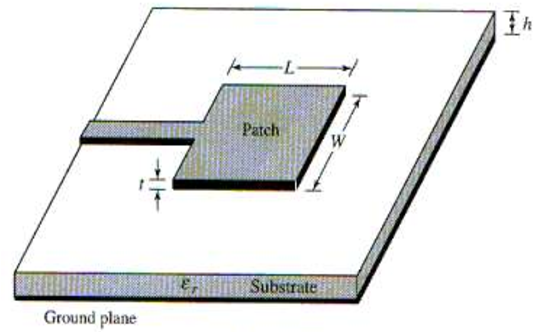
\includegraphics[width=0.5\textwidth]{patch-antenna-structure.png}
    %\end{subfigure}
    \caption{The basic structure of a patch antenna. This particular antenna is being fed with a microstrip. The ground, and the patch are conductors. The substrate is a dielectric. \cite{girase2014design}}
\end{figure}

Besides its large size at lower frequencies, a PA with Figure 1's design would have a narrow frequency band, low efficiency, low power, high Q, poor polarization purity, and spurious feed radiation\cite{balanis2016antenna}. Fortunately, significant effort has gone into addressing these limitations, and a variety of design techniques to mitigate these limitations have been created\cite{balanis2016antenna}. Furthermore, PAs have also been investigated theoretically, and theories to describe the operating mechanism of most PAs have been created. However, the theories describing PA operation are mathematically dense, and are quite challenging to read. This unapproachability in theory leads to obfuscation on both the theory of PA operation, and research associated with it. One of the most intuitive high level ways of describing antennas is visually. While antenna simulation software does exist, it seems like nobody has used it provide a surface level introduction to patch antennas. This paper intends to do so, using the antenna simulation software known as HFSS, by Ansys. HFSS is a 3D electro-magnetic field simulator, used by RF engineers to design antennas, but it can also be used to visualize the fields in patch antennas, thereby giving an intuitive explanation of why certain antenna designs work, and others don't.

This paper will use HFSS to provide a visual explanation of the radiation mechanism of a basic PA, as well as show some of its properties. Afterwards, the paper will review some methods which have been used to miniaturize PAs. None of the presented methods will be exceptionally novel, however, the methods are actually used in current patch antennas, and the mechanism behind their operation is fascinating in its own right. Since this is a surface level paper, certain concepts will be introduced without adequate in depth explanation. In these cases, the paper will reference other readings for a more in depth explanation.            
  
\section{Electromagnetic Radiation}  

Before discussing patch antennas, it is important to understand how electromagnetic radiation is created in the first place. Unlike light bulbs, which generate light via the energy released by electrons decaying to lower energy levels inside atoms, antennas radiate via a completely different principle.

Consider a pair of positive and negative electric charges, with some distance $d$ between them. For the sake of this example, also suppose that the two charges are somehow held in place. If this didn't happen, then the two charges would immediately attract together. Consider the electric field created by these two charges. As shown in figure 1, the electric field lines go from the positive charge to the negative charge, in a dilpole fashion.

\begin{figure}[h]
    %\begin{subfigure}{0.5\textwidth}
    \centering
    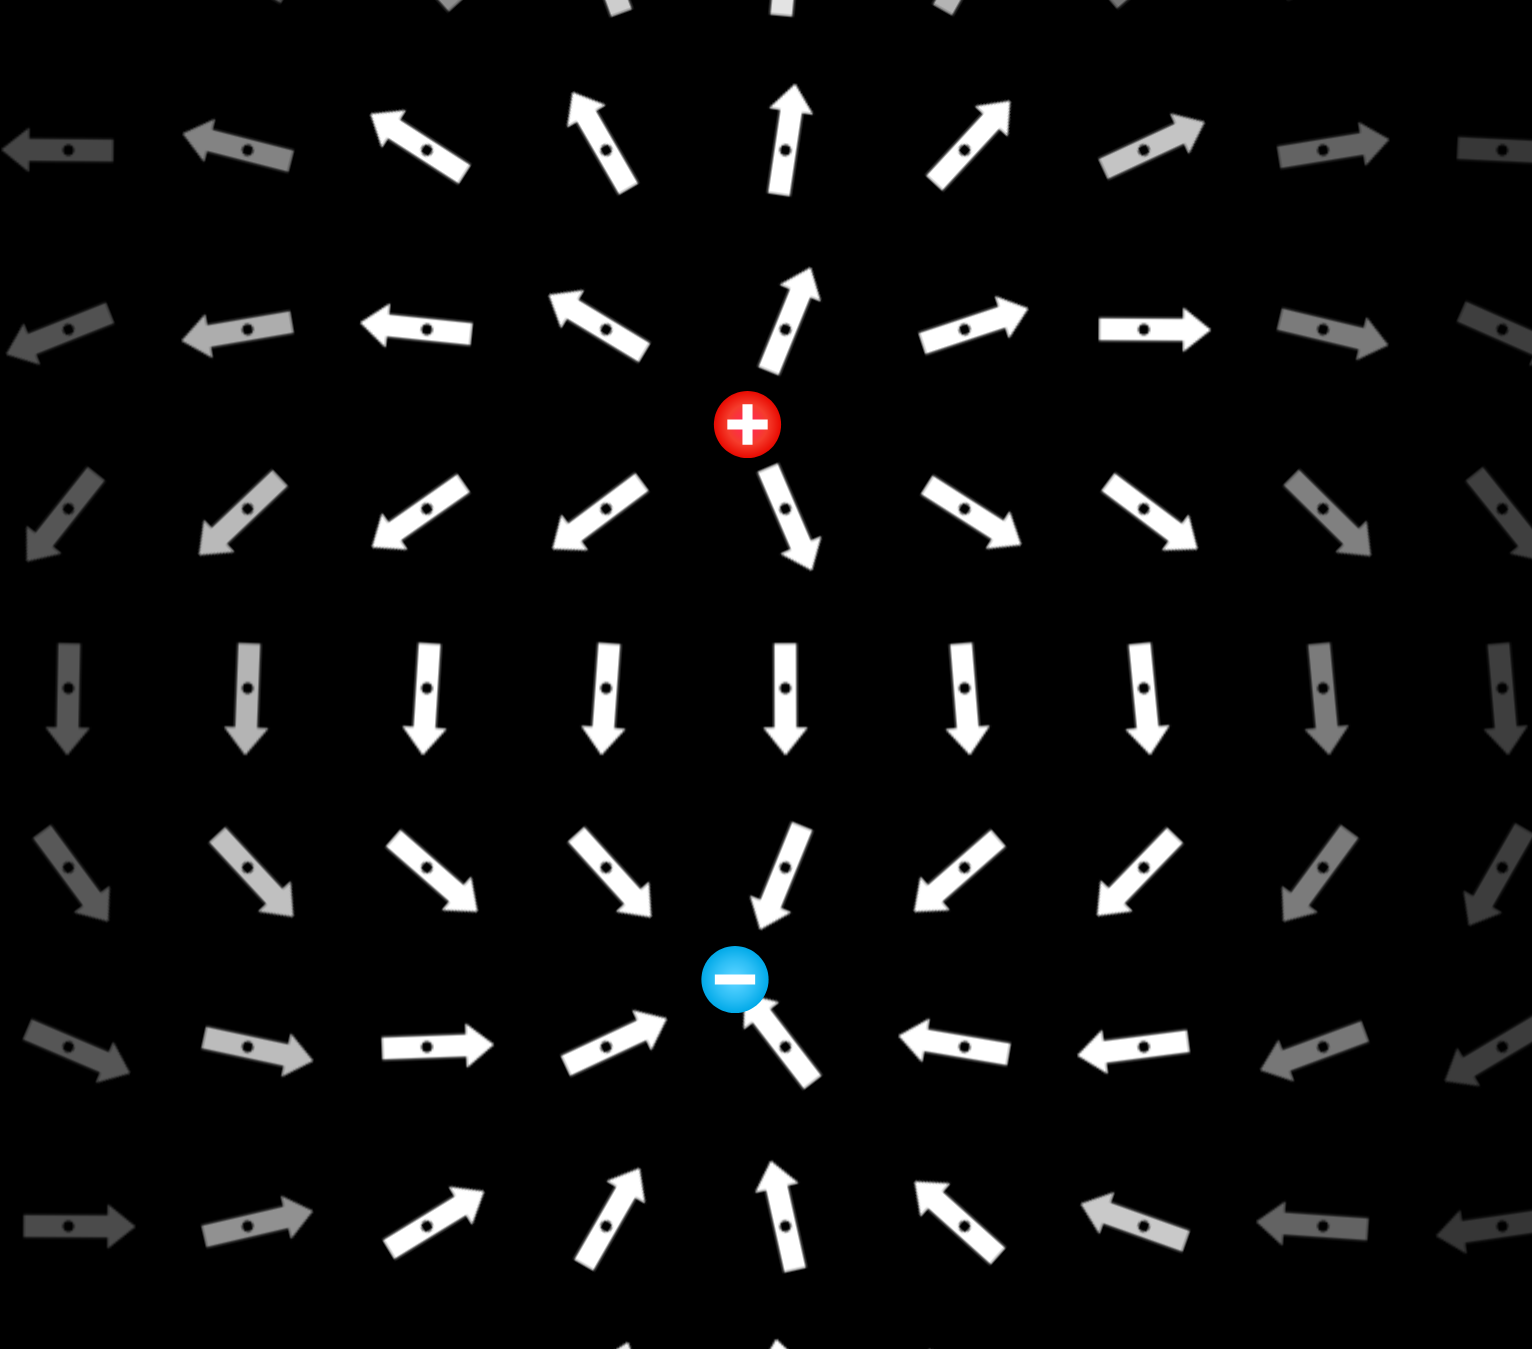
\includegraphics[width=0.3\textwidth]{positive-negative-EField.png}
    %\end{subfigure}
    \caption{The electric field around two point charges of equal magnitude, but of opposite sign.}
\end{figure} 

Now, consider what happens to the E-field around the charge when the charge is moving at some velocity $v$. One would expect that the field around this moving charge would look something like in figure 2, in the reference frame of a stationary observer. This is not correct, even if $v = 0.9c$.

\section{Properties of Alternating Current}

\section{Patch Antenna}

\subsection{Basic Characteristics}
As shown in figure 1, a basic patch antenna consists of a very thin metallic strip (the patch), placed a small fraction of a wavelength above a metallic ground plane. While patches are usually either rectangular or circular\cite{khan2015microstrip}, numerous other shapes have been investigated\cite{balanis2016antenna}. In between the patch, and ground plane, is a dielectric. Dielectrics are electronic insulators which can be polarized by an external electric field. 

\begin{figure}[h]
    %\begin{subfigure}{0.5\textwidth}
    \centering
    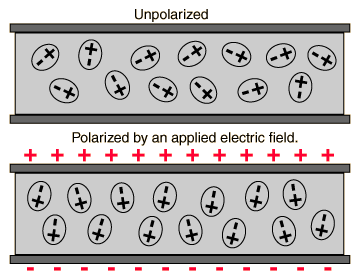
\includegraphics[width=0.3\textwidth]{dielectric.png}
    %\end{subfigure}
    \caption{ [Uncited, provide a citation here] A dielectric with and without an applied E-field. The dielectric constant $\epsilon_r$ (relative permittivity) is a measure of how much the atoms in the dielectric align to the external E-field. Dielectrics with low $\epsilon_r$ will polarize less to the external E-field, compared to high $\epsilon_r$ dielectrics.}
\end{figure}

Numerous dielectric materials are used in PAs. Most of these materials will have dielectric constants in the range of $2.2$ to $12$\cite{balanis2016antenna}. More discussion on the choice of substrate in the antenna will be provided in section 3. 
\section{Radiation Mechanisms}

The three most popular model used to describe patch antennas are, the transmission line model, the cavity model, and the full wave model\cite{balanis2016antenna}. Since the transmission line model gives the best visual insight\cite{balanis2016antenna} into patch antenna operation, this model will be used. It should be noted however, that the transmission line model is only valid for rectangular patch antennas, and doesn't give the most accurate results\cite{balanis2016antenna}. As a result, the results from both the cavity wave model, and the full wave model will be included. More information on the cavity model can be found here \cite{balanis2016antenna}. 


\section{E-Field on the Patch}
 

\begin{figure}[h]
    %\begin{subfigure}{0.5\textwidth}
    \centering
    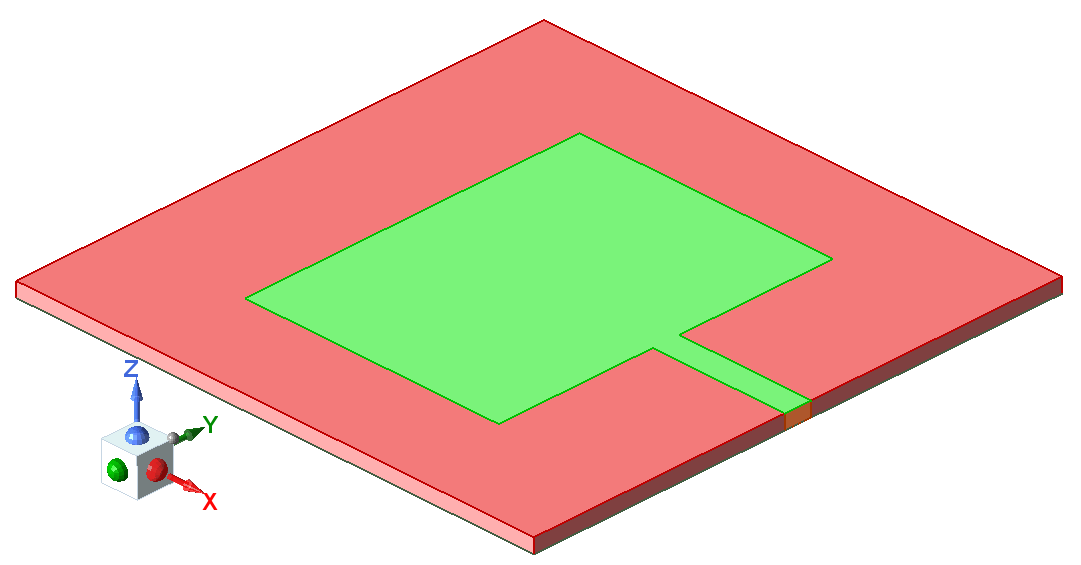
\includegraphics[width=0.5\textwidth]{2.4GHz-basic-pa.png}
    %\end{subfigure}
    \caption{A basic PA designed in HFSS. This particular PA has been designed to radiate at 2.4 GHz. The green material on top is the patch, with the red material being the substrate. The substrate has a relative permittivity (dielectric constant) of 4.4. There is a ground plane beneath the substrate, although it is not visible here. The entire antenna has dimensions $60 \text{ mm} \times 60 \text{ mm} \times 1.6 \text{ mm}$, in the x,y,z planes, respectively. The patch itself is 29.4 mm long in the x direction, and 38 mm long in the y direction. The thickness of the patch and ground plane is negligible with respect to the substrate thickness. }
\end{figure}

Figure 3 depicts a basic microstrip patch antenna (MPA) that is designed to radiate at 2.4 GHz. When an RF signal is applied to this antenna, at a 2.4 GHz frequency, the patch antenna will radiate EM waves. Although the antenna can radiate at other frequencies, it will radiate less efficiently at those frequencies. The frequency at which an antenna radiates most efficiently is known as the \textit{resonant frequency} of the antenna. A more technical definition of the resonant frequency of an antenna is the frequency at which the impedence of an antenna is purely resistive, the frequency at which the capacitive and inductive reactances cancel each other out. 

The exact radiation mechanism for a rectangular patch antenna can be modeled by treating the patch as an open ended transmission line. When a signal passes through the micro-strip and into the patch itself, the signal travels down the length of the patch, and is reflected upon reaching the far end of the patch. The reflected signal then interferes with the incoming RF signal, to create a standing wave on the patch. This standing wave then allows for the radiation of free space waves. The reflected signal does not travel back into the micro-strip and into the feedline due to the impedence mismatch between the microstrip line and the patch. So, when the reflected signal reaches the other side of the patch, it gets reflected again, and will be reflected until it runs out of energy.   

\begin{figure}[h]
    %\begin{subfigure}{0.5\textwidth}
    \centering
    \includegraphics[width=0.5\textwidth]{basic-patch-antenna-MagE-on-patch.png}
    %\end{subfigure}
    \caption{This depicts the same PA from figure 3, with an RF current applied to the patch. The magnitude of the E-field is being shown on the patch, with the RF current applied. A stronger E-field at some point is represented by a warmer color.}
\end{figure}

As observed in figure 4, the E-field is strongest around the edges of the patch, and decreases rapidly towards the center of the patch. This is due to the skin effect, where at either high frequencies, or high currents, the current through a conductor gets pushed out to the outermost edges. 

\begin{figure}[h]
    %\begin{subfigure}{0.5\textwidth}
    \centering
    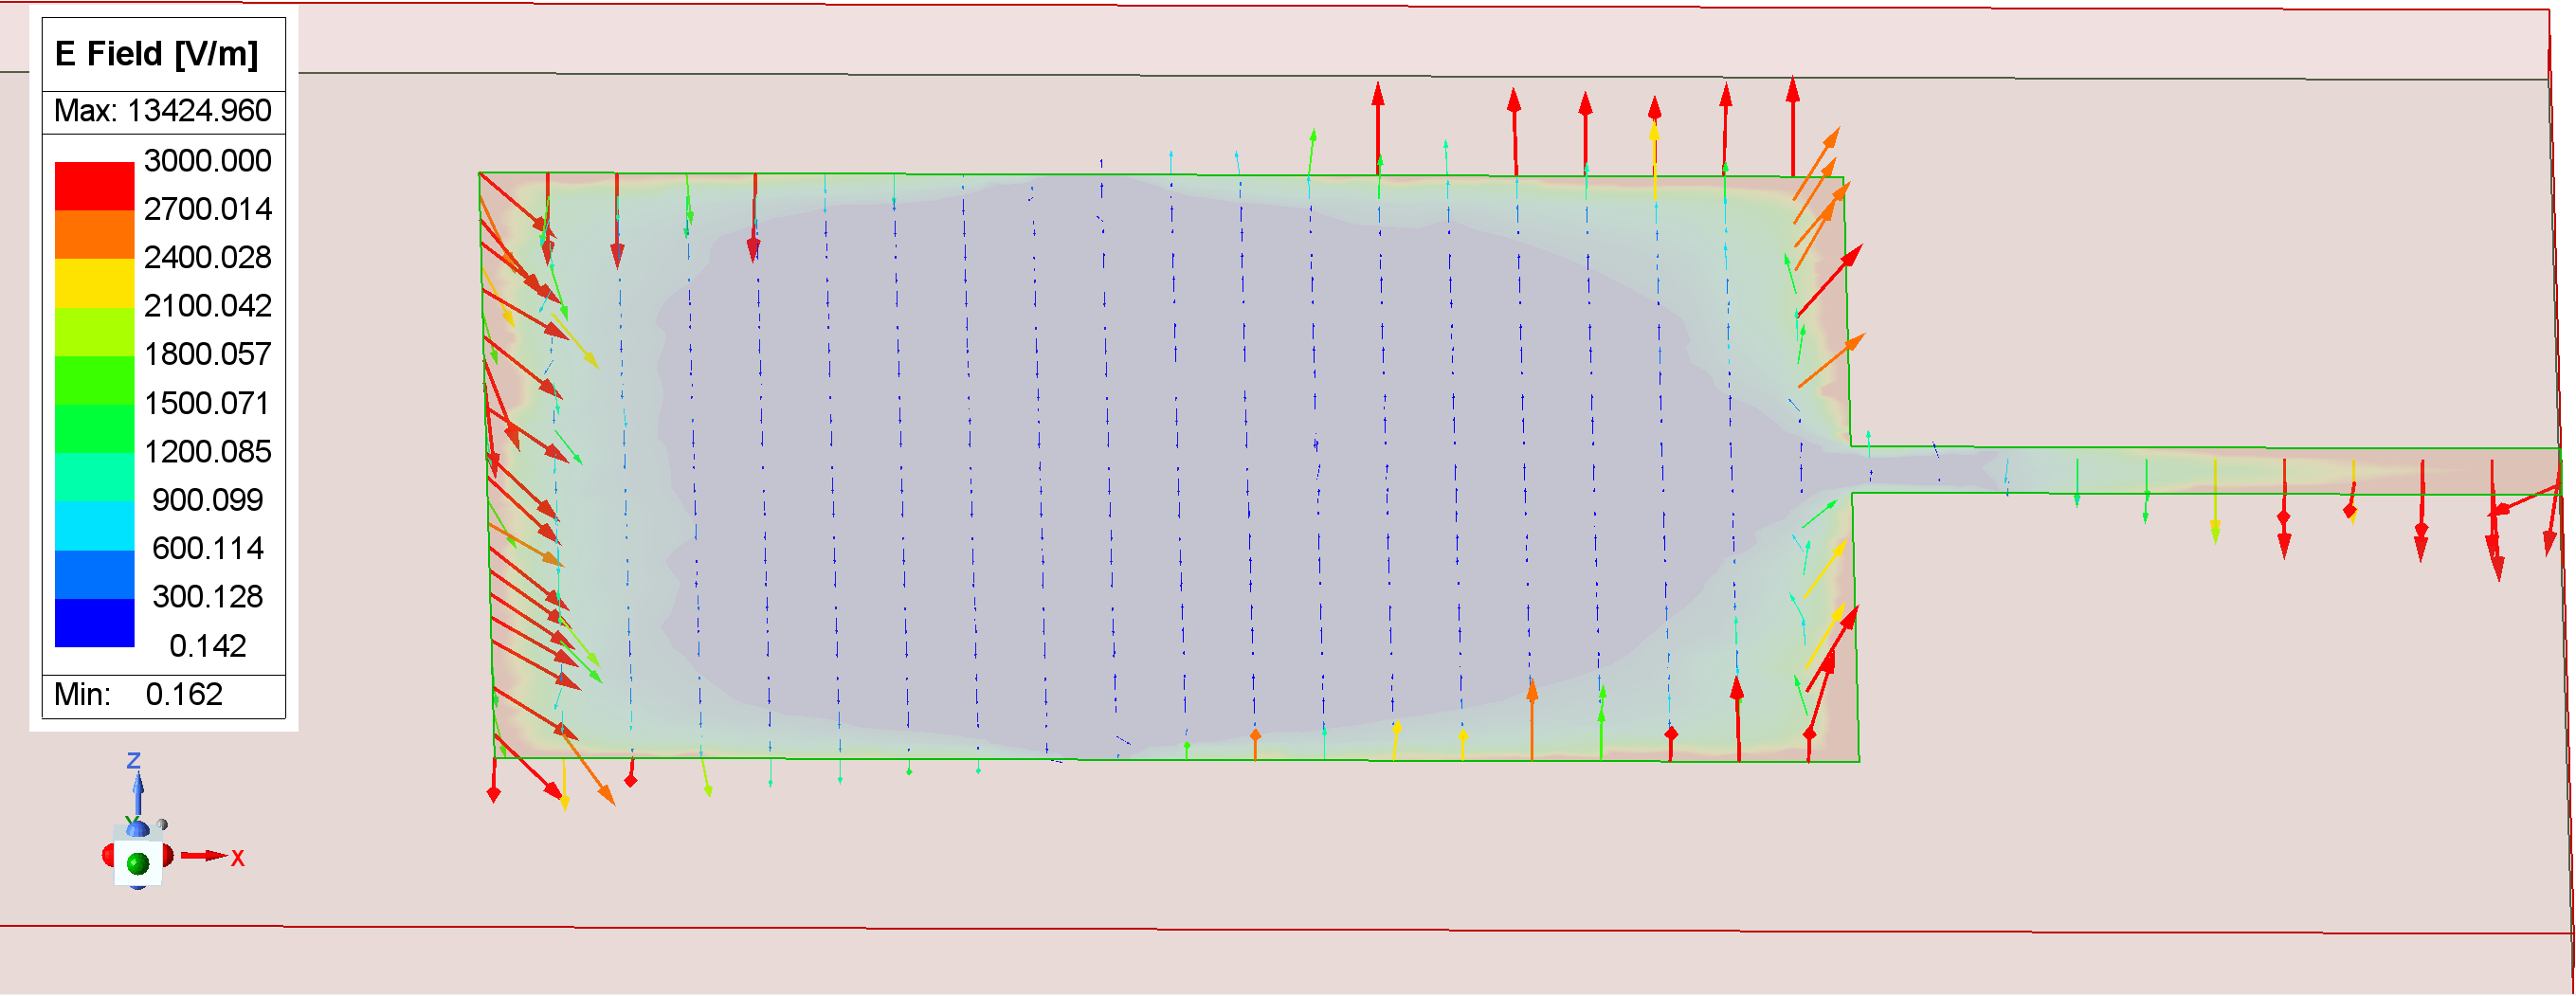
\includegraphics[width=0.5\textwidth]{basic-patch-antenna-VecE-onPatch-t0.png}
    %\end{subfigure}
    \caption{This shows the E-field as a vector on the patch. It is clear that the E-field is strongest on the outside edge of the patch, while the center of the patch has virtually no E-field. Furthermore, the E-field at either end of the patch is not oriented solely in the z direction, which is due to the curvature of the edge of the patch.}
\end{figure}

Although figure 5 clearly shows that the E-field is strongest at the close and far ends of the patch, and that they mostly point in the direction parallel to the z-axis, it raises another important question: why are the fields pointing in the same direction with respect to the x-axis? To answer this question, consider the E-field near the patch.  

\section{Near Field Radiation}

To better understand the far field radiation pattern of the patch, first consider the E-field pattern around the patch. As demonstrated in figure 5, the edges of the patch contain the strongest E-field. Consider what would happen if the sources of these strong E-fields was fixed. As time passes, the new surrounding space would conform to these E-fields. An important realization is that the two locations where the E-fields are strongest can be modeled as a pair of opposite electric charges. At a certain distance the E-field will point from one point of strong E-field, to the other point of strong E-field, as shown in figure 6.

\begin{figure}[h]
    %\begin{subfigure}{0.5\textwidth}
    \centering
    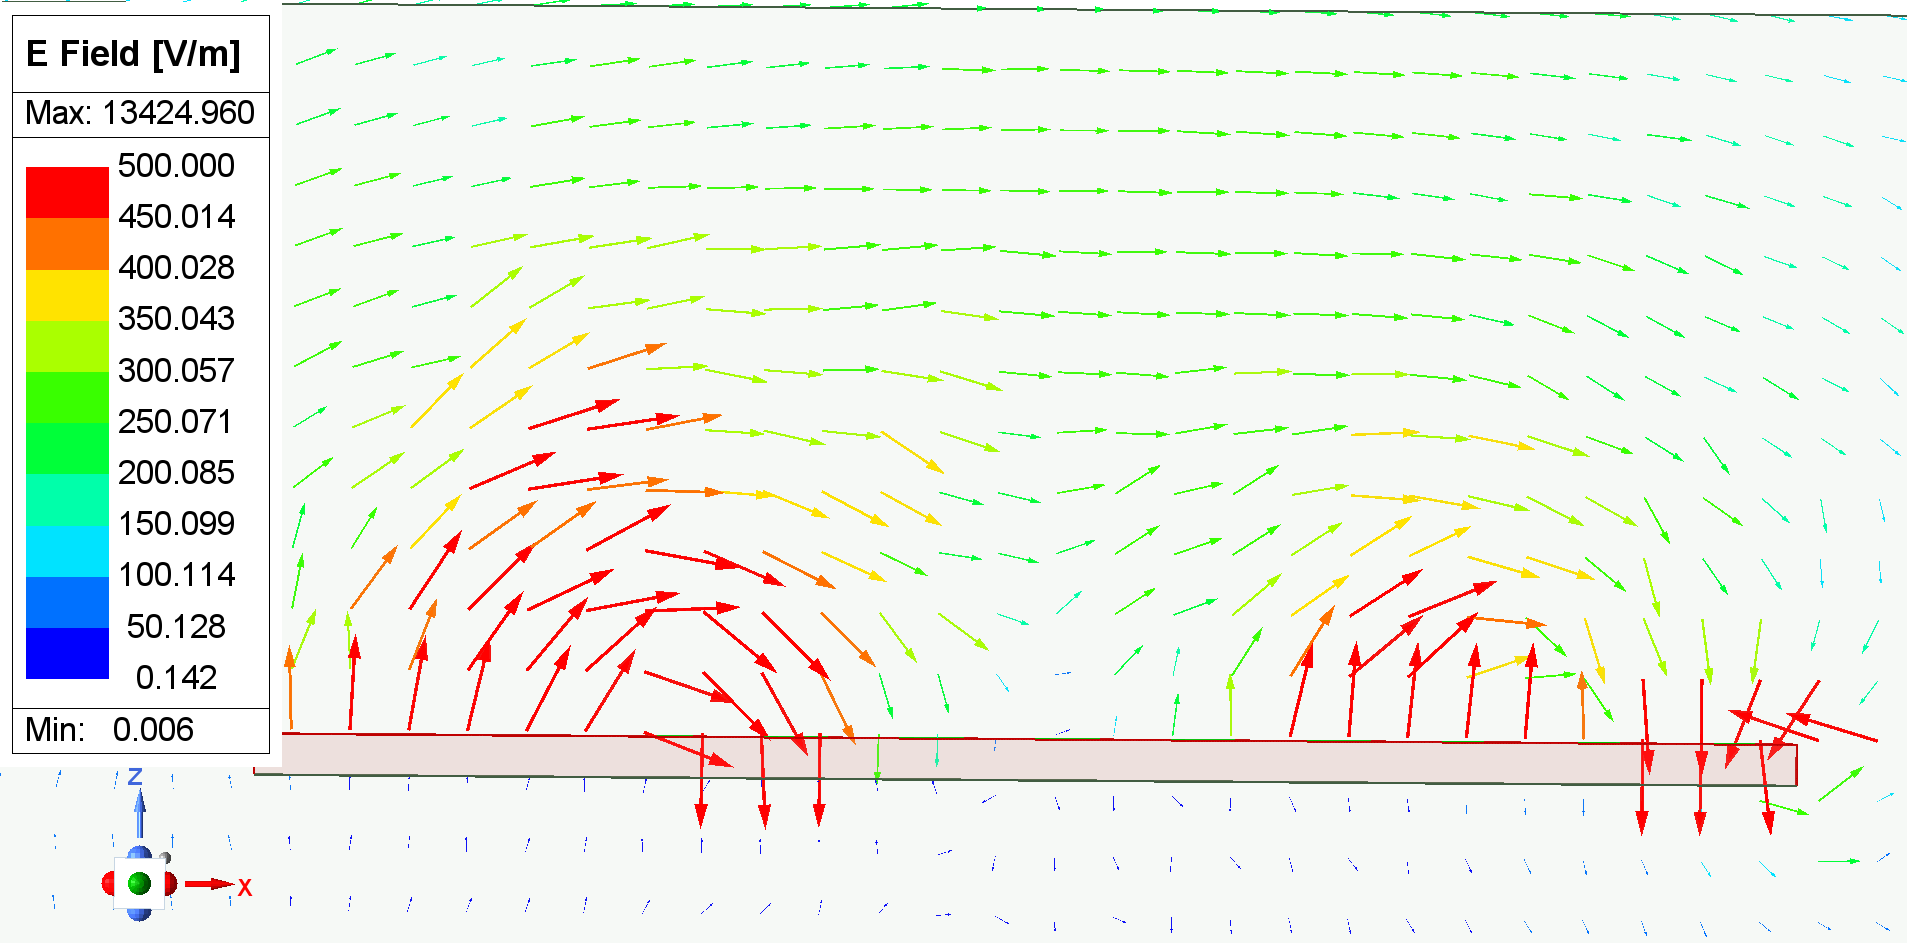
\includegraphics[width=0.5\textwidth]{basic-patch-antenna-near-Efield.png}
    %\end{subfigure}
    \caption{This shows the E-field near the patch, at a snapshot in time. Observe that at a certain distance the E-field appears to travel from one point of high E-field strength to the other. In other words, from a certain distance the overall pattern of the E-field matches the expected pattern of an E-field formed by a positive and negative pair of charges.}
\end{figure}  
This connected E-field will extend out towards infinity (assuming that the charges remain fixed), and is crucial to understanding the far field radiation of the antenna. 

\section{Far Field Radiation}

As demonstrated previously, the two opposite E-fields create a surrounding E-field similar to that of an electric dipole. But notice that the E-field on the patch is constantly oscillating back and forth, and so, the 

\begin{figure}[h]
    \begin{subfigure}{0.5\textwidth}
    \centering
    	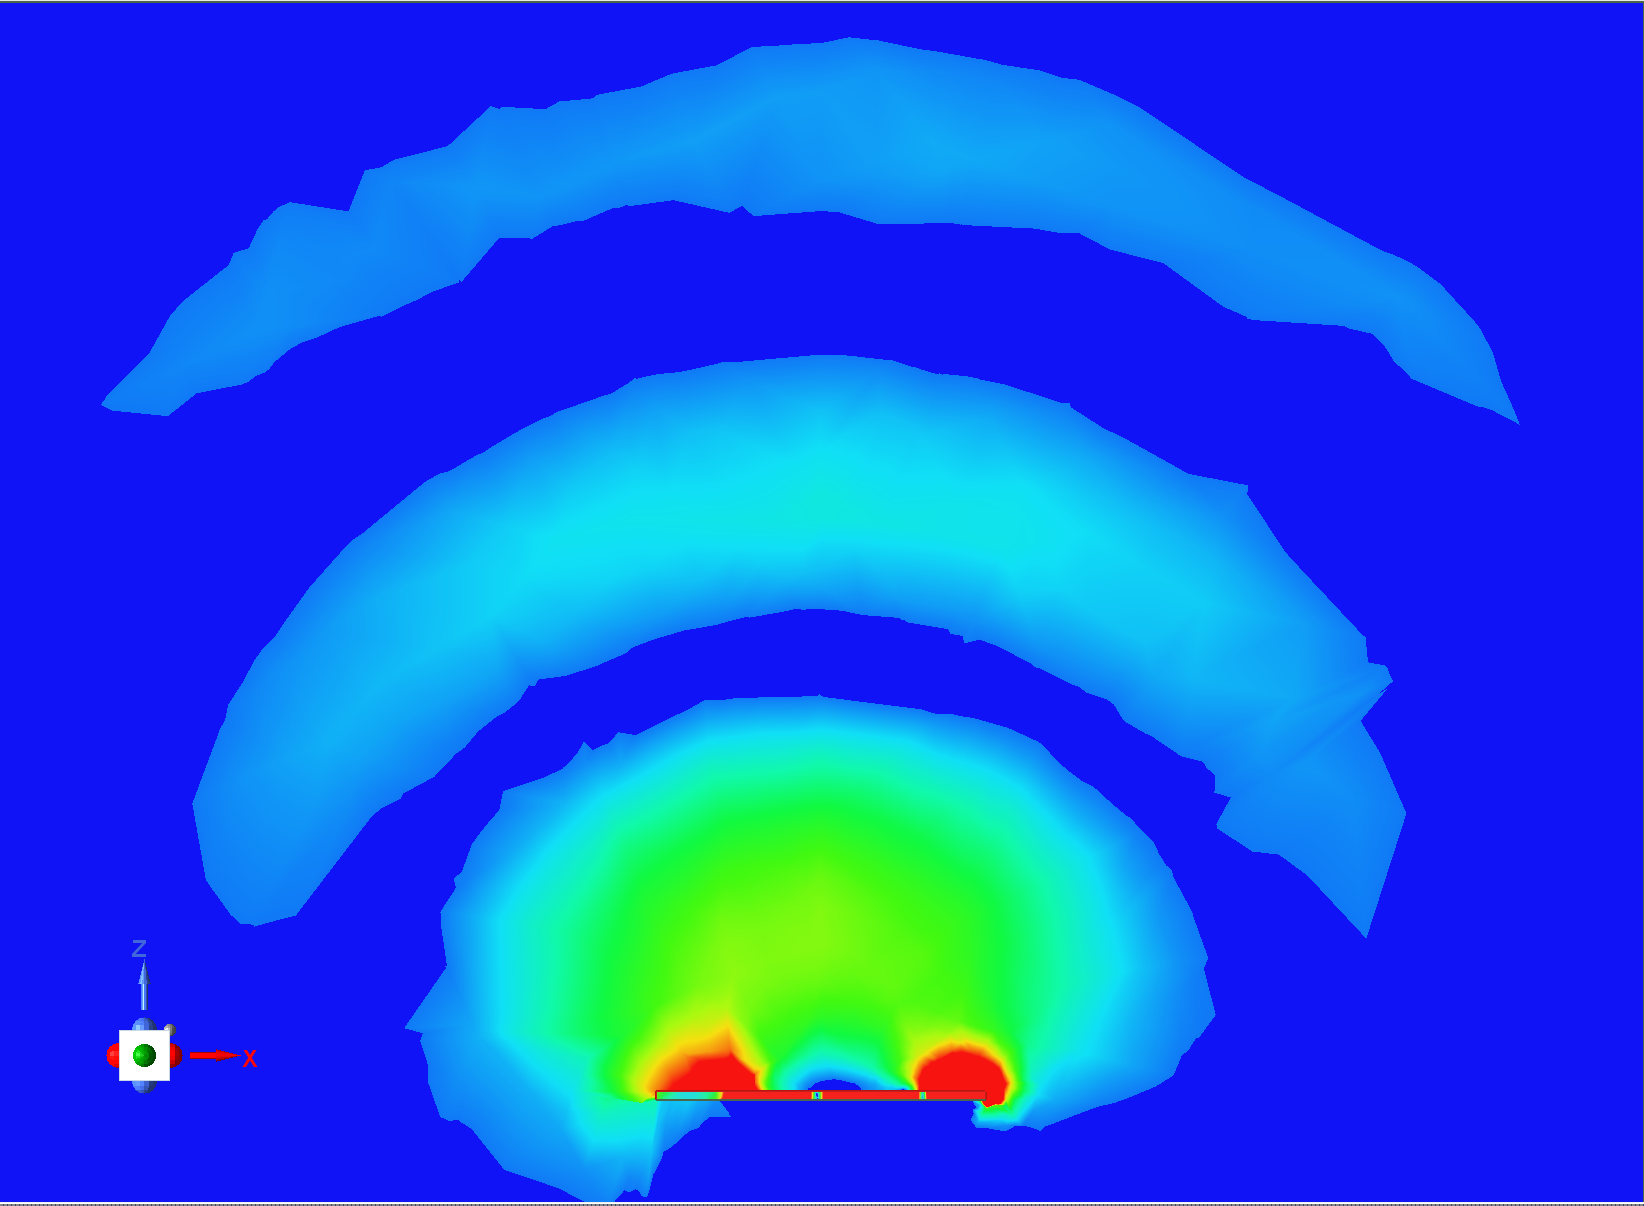
\includegraphics[width=0.5\textwidth]{basic-patch-antenna-radiating-t0.png}
    \end{subfigure}
    \begin{subfigure}{0.5\textwidth}
    \centering
    	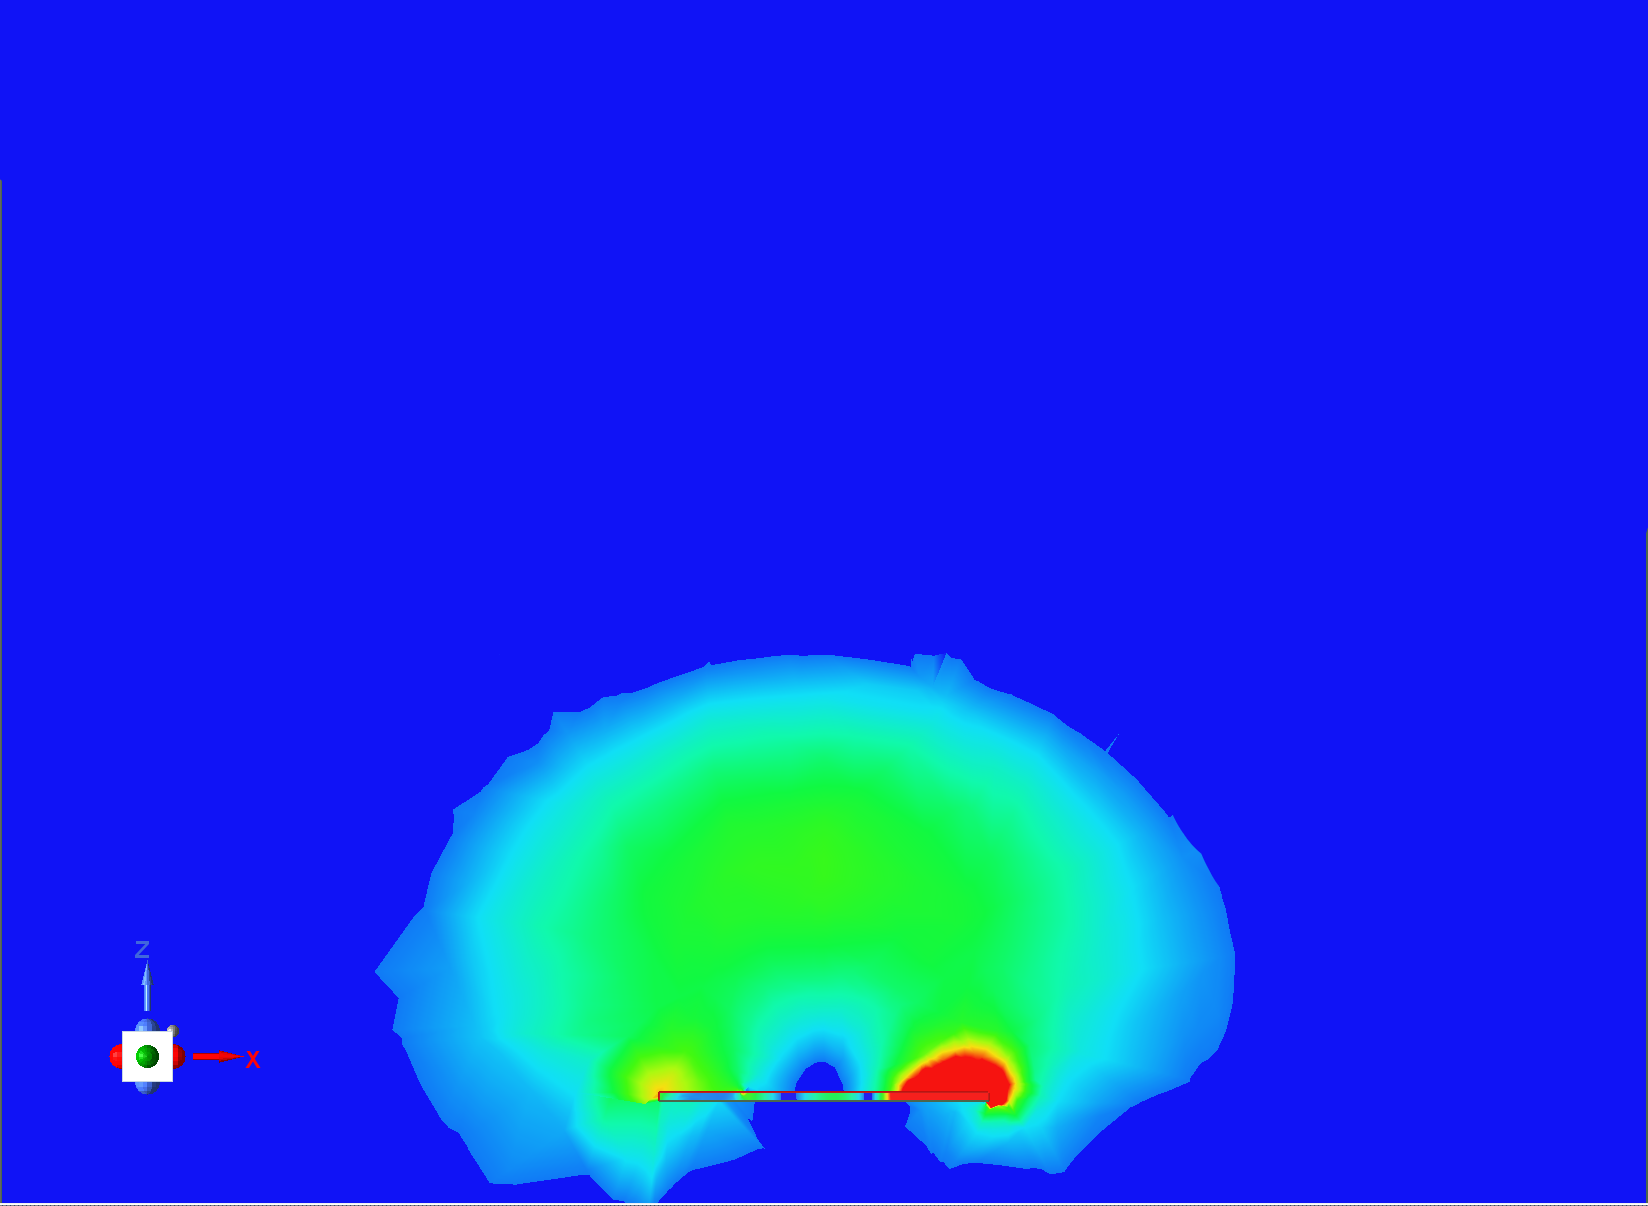
\includegraphics[width=0.5\textwidth]{basic-patch-antenna-radiating-t1.png}
	\end{subfigure}   
    \begin{subfigure}{0.5\textwidth}
    \centering
    	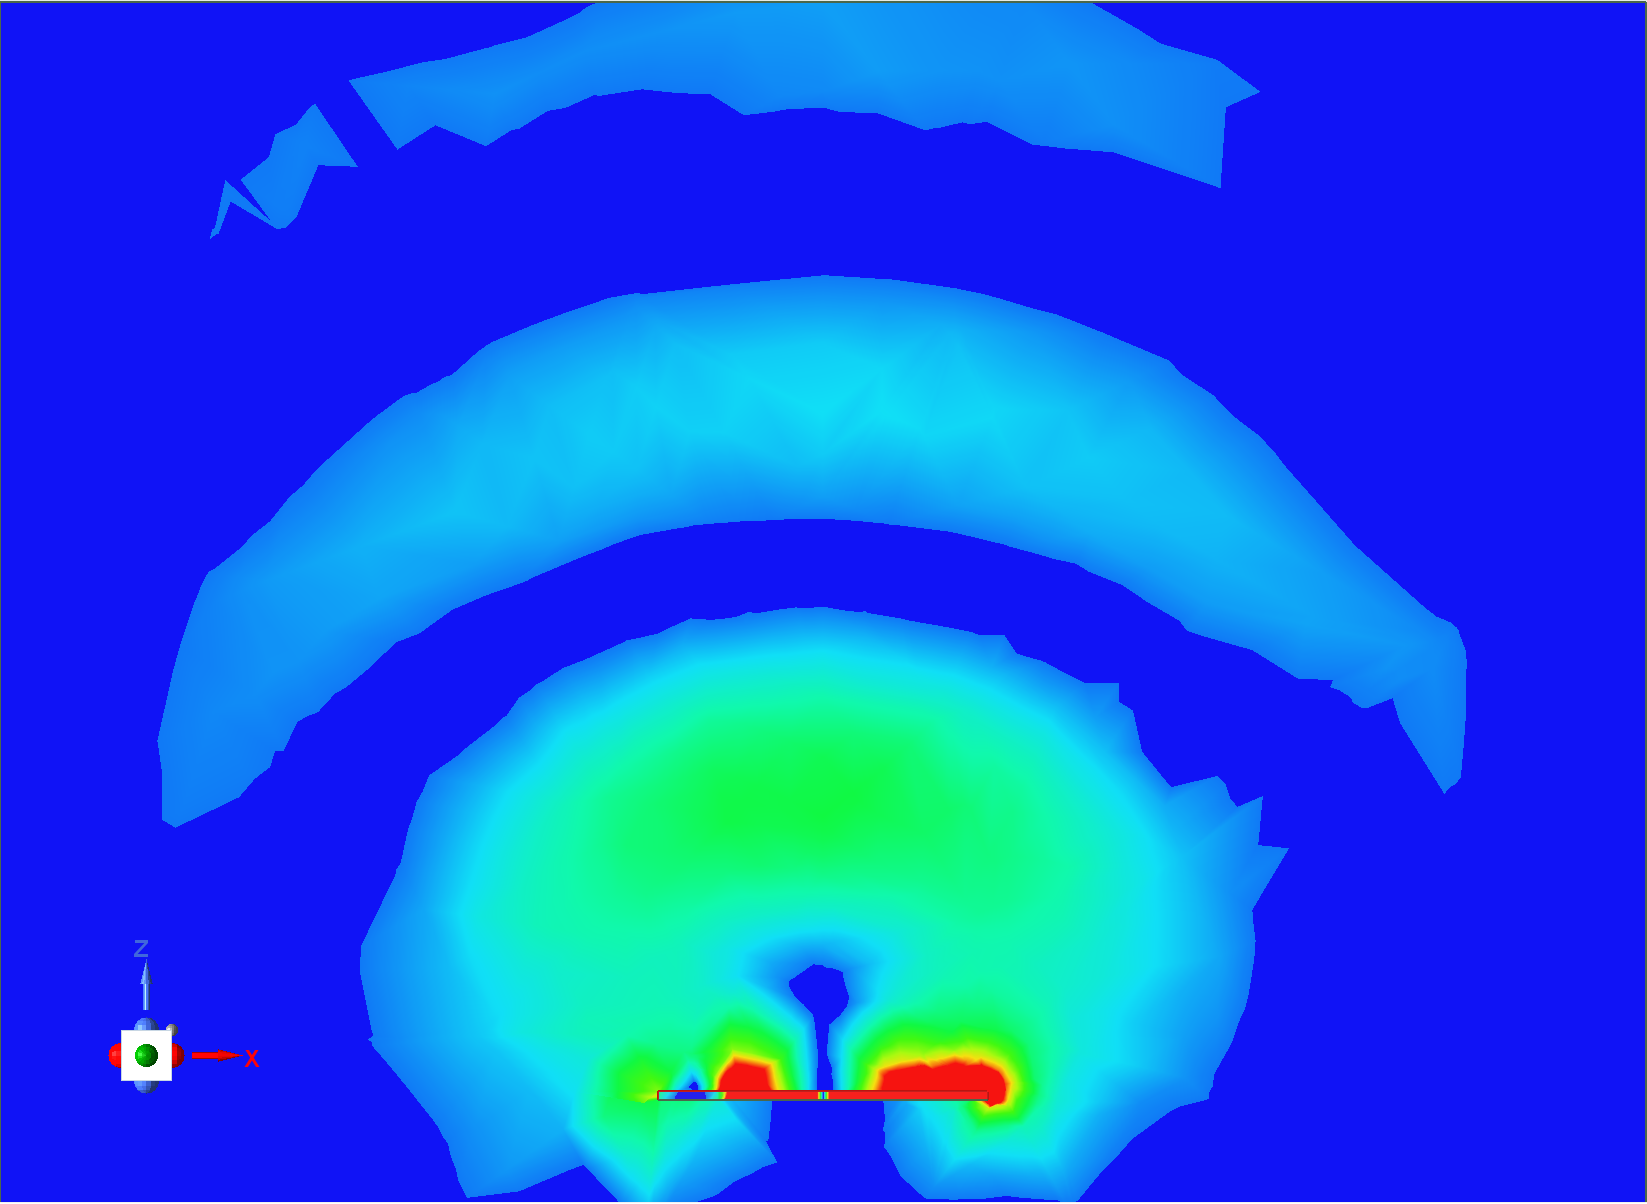
\includegraphics[width=0.5\textwidth]{basic-patch-antenna-radiating-t2.png}
	\end{subfigure}    
    \begin{subfigure}{0.5\textwidth}
    \centering
    	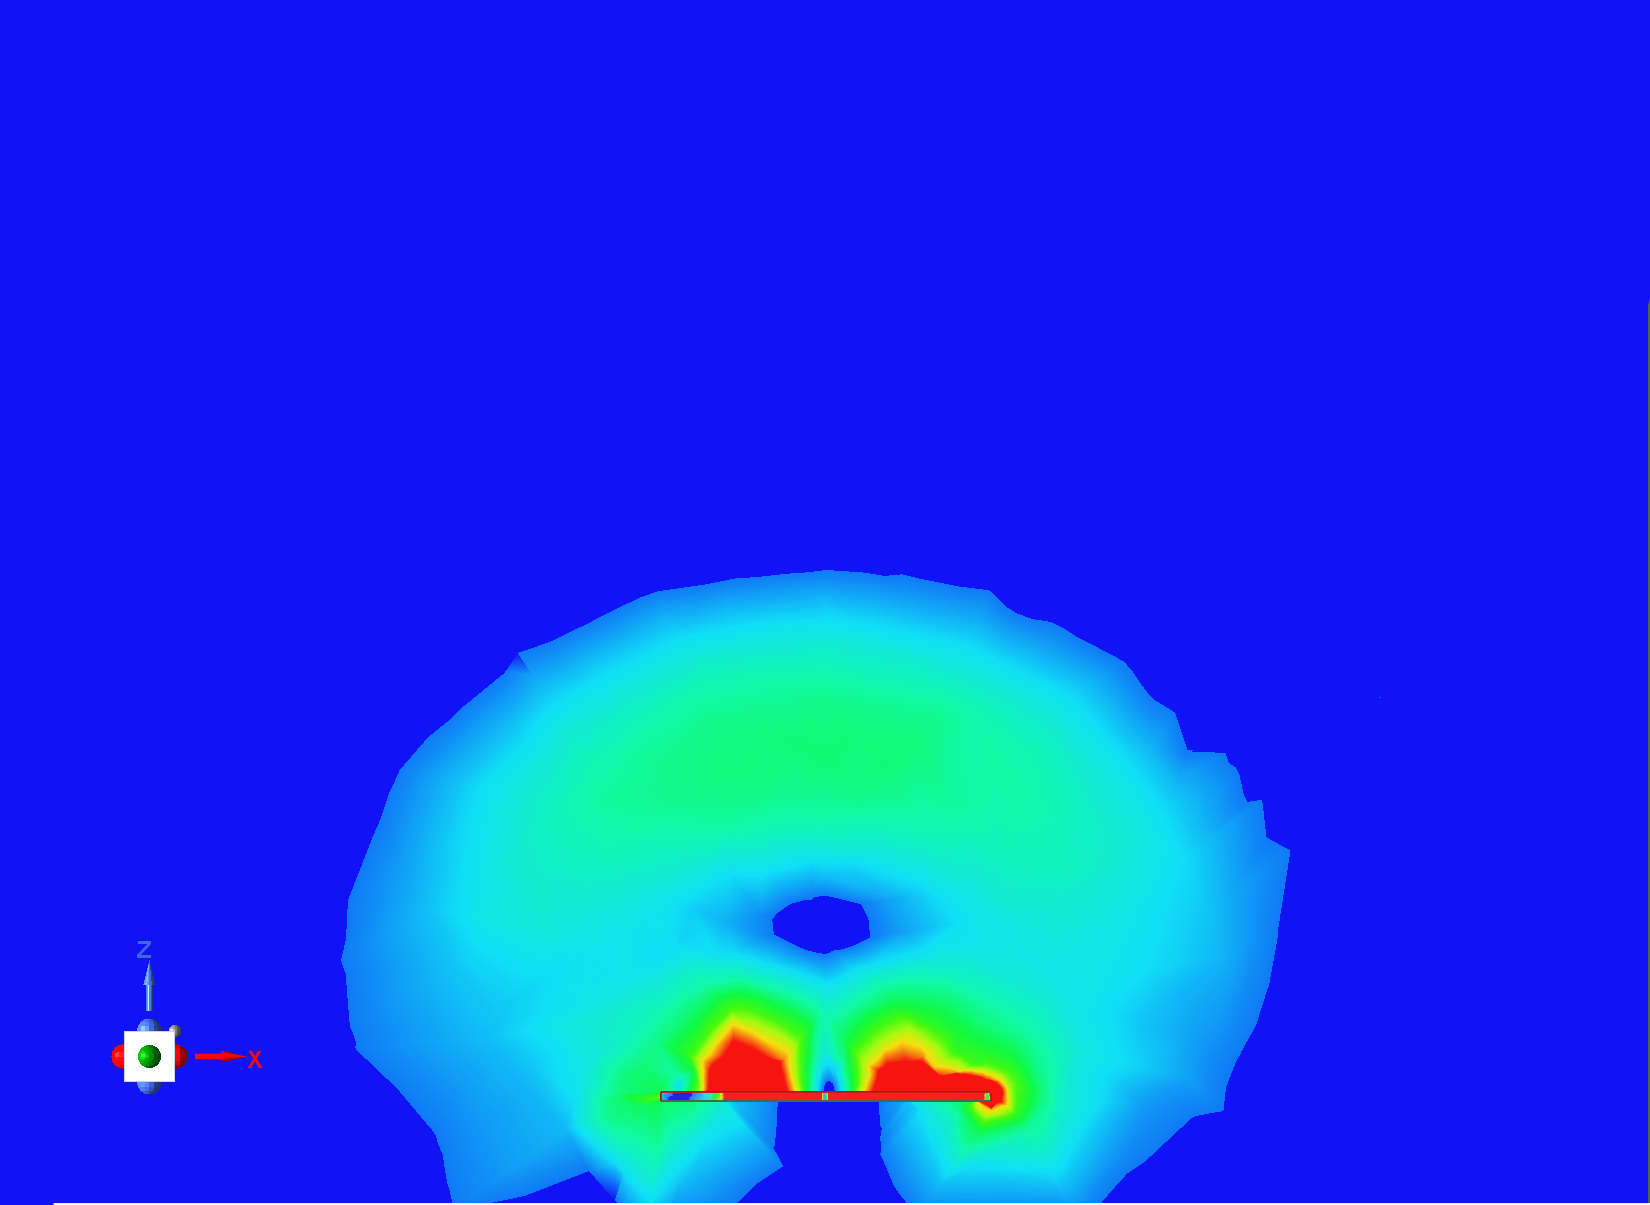
\includegraphics[width=0.5\textwidth]{basic-patch-antenna-radiating-t3.png}
    \end{subfigure}
    \begin{subfigure}{0.5\textwidth}
    \centering
    	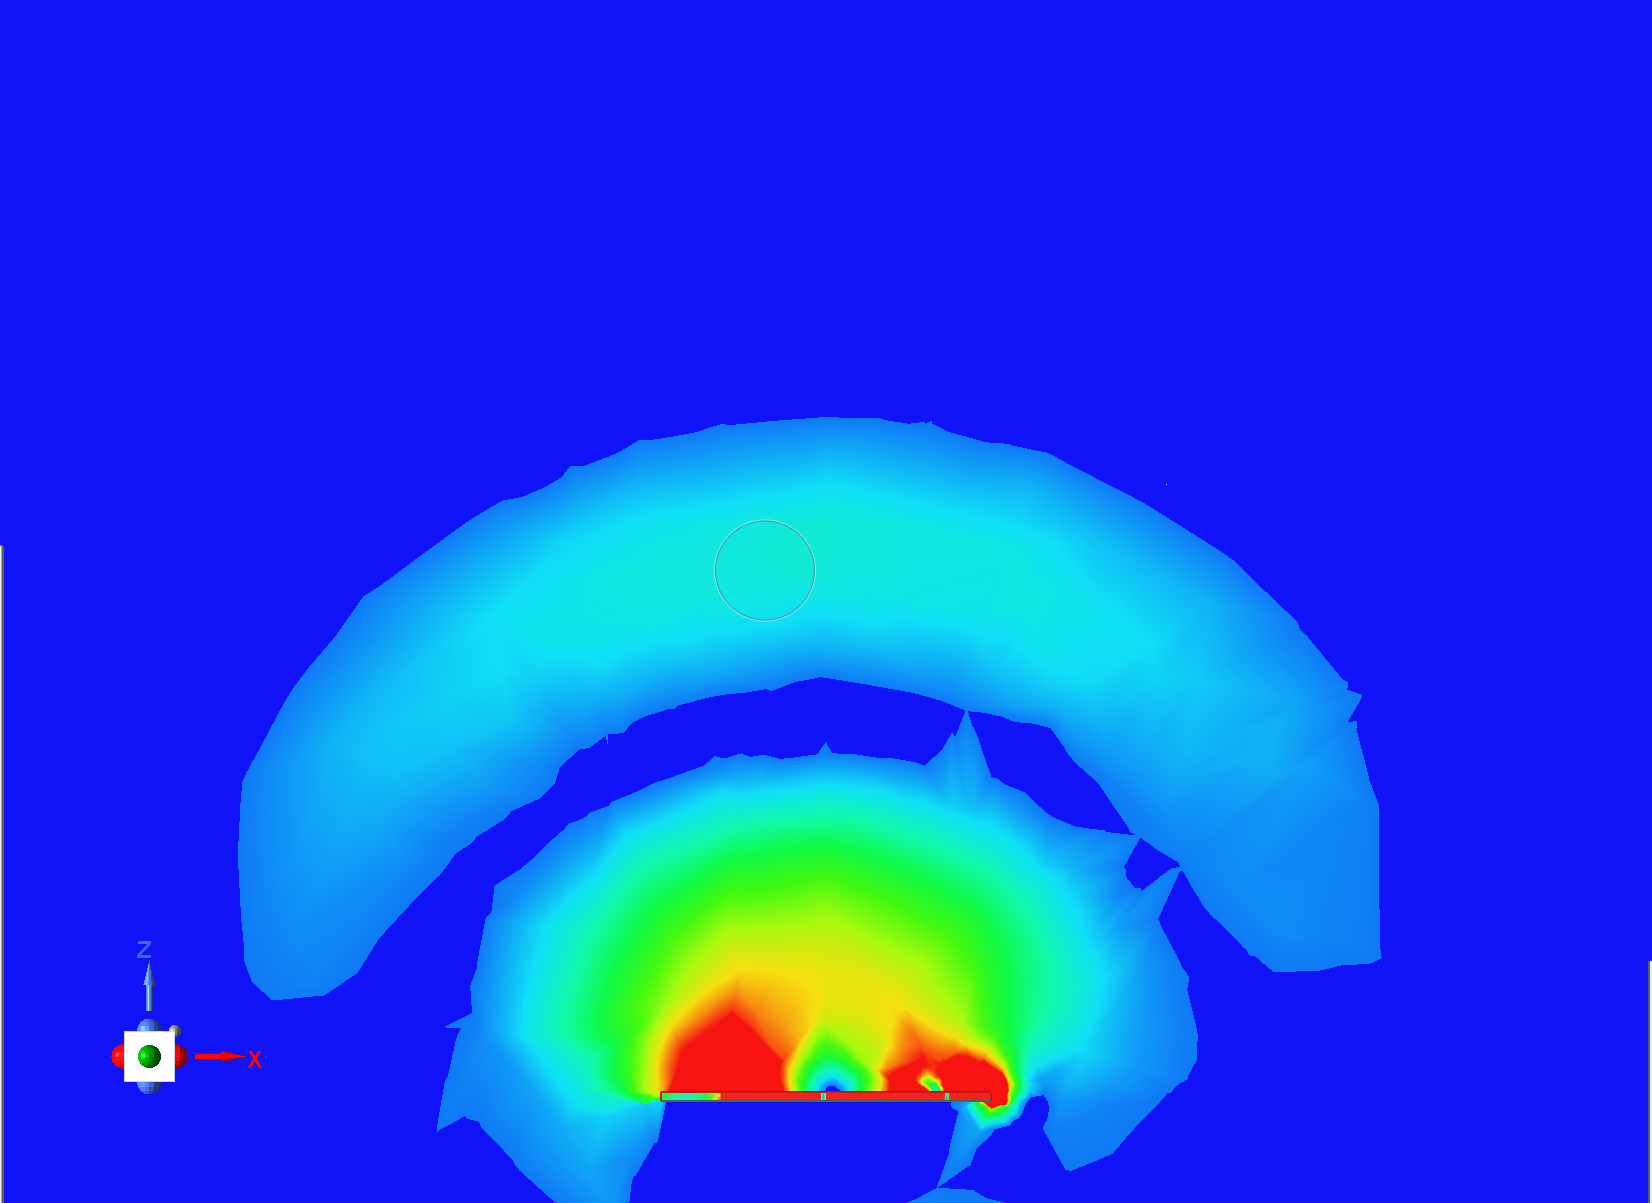
\includegraphics[width=0.5\textwidth]{basic-patch-antenna-radiating-t4.png}
    \end{subfigure}
    \caption{This shows the E-field near the patch, at a snapshot in time. Observe that at a certain distance the E-field appears to travel from one point of high E-field strength to the other. In other words, from a certain distance the overall pattern of the E-field matches the expected pattern of an E-field formed by a positive and negative pair of charges.}
\end{figure}  

\section{Properties}

\section{Conclusion}

\newpage
\bibliographystyle{IEEEtran}
\bibliography{main}
%\printbibliography


\end{document}
